\documentclass[xcolor=dvipsnames]{beamer}
\usepackage[utf8]{inputenc}
\usepackage{lmodern}
\usepackage[T1]{fontenc}
\usepackage[numbered,framed]{matlab-prettifier}

\usepackage{xcolor}
\usepackage{mathtools}
\makeatletter
\newcommand*\colvec[3][]{
    \begin{pmatrix}\ifx\relax#1\relax\else#1\\\fi#2\\#3\end{pmatrix}
}
\newcommand{\redub}{}
\def\redub#1{%
  \@ifnextchar_%
    {\@redub{#1}}
    {\@latex@warning{Missing argument for \string\redub}\@redub{#1}_{}}%
}
\def\@redub#1_#2{%
    \colorlet{currentcolor}{.}%
    \color{red}%
    \underbrace{\color{currentcolor}#1}_{\color{red}#2}%
    \color{currentcolor}%
}
\makeatother

\newsavebox{\firstexample}
\newsavebox{\findroot}
\newsavebox{\original}
\usetheme{lankton-keynote}
\setbeamercolor{title}{fg=White}
\setbeamercolor{frametitle}{fg=White}
\let\ph\mlplaceholder % shorter macro
\lstMakeShortInline"
\lstset{
  style              = Matlab-editor,
  basicstyle         = \mlttfamily,
  escapechar         = ",
  mlshowsectionrules = true,
}

\author{Christopher Lillthors Viktor Kronvall}
\title{Pilbågen}

\begin{document}
\maketitle
\setbeamertemplate{frametitle}[default][center]

%define MATLAB-code boxes.
\begin{lrbox}{\firstexample}
\begin{lstlisting}[caption=Föreklat system]
   y = @(x) 0.3*cos(x*q_sqrt);
   y_ = @(x) -0.3*q_sqrt*sin(x*q_sqrt);
   f = @(t,u) [y_(t);-q*y(t)];
   u = [0.3 0];
   [xs, ys] = ode45(f, [0 a], u);
\end{lstlisting}
\end{lrbox}

\begin{lrbox}{\findroot}
\lstinputlisting{../labb3/findroot.m}
\end{lrbox}
\begin{lrbox}{\original}
\lstinputlisting{../labb3/ursprunglig.m}
\end{lrbox}

% slide 1
\begin{frame}
\frametitle{Problem}
\begin{figure}[h!]
\centering
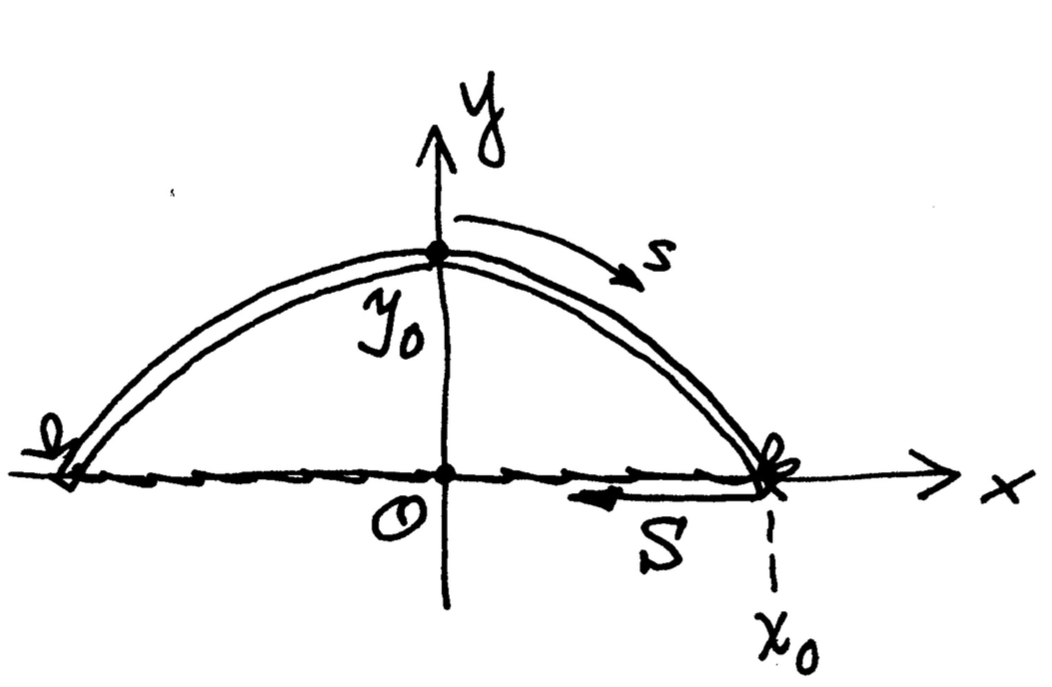
\includegraphics[scale=0.2]{bild.png}
\end{figure}
\end{frame}

% slide 2
\begin{frame}
\frametitle{Problem}
\begin{figure}[h!]
\centering
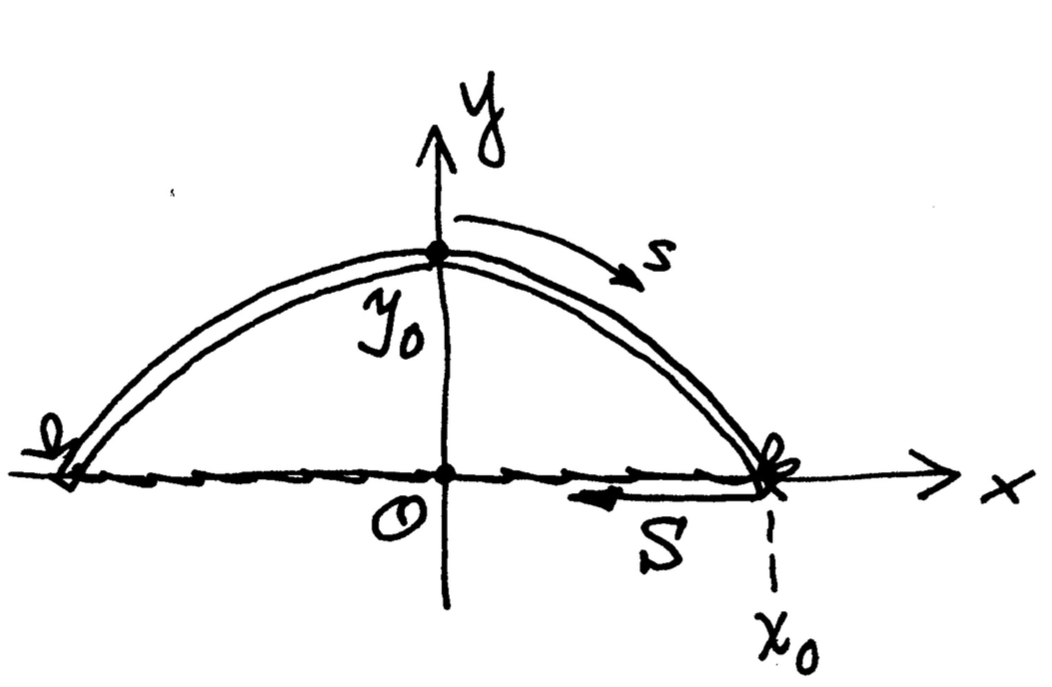
\includegraphics[scale=0.1]{bild.png}
\end{figure}
\begin{equation} \label{eq:original}
	\dfrac{d^2y}{dx^2} + qy \left(1+\left(\dfrac{dy}{dx}\right)^2\right)^{3/2} = 0 \nonumber
\end{equation}
\begin{equation}
s = \int_0^a{\sqrt{1+y'(x)^2}}=0.5 \nonumber
\end{equation}
\end{frame}

% slide 3
\begin{frame}
\frametitle{Problem}
\begin{figure}[h!]
\centering
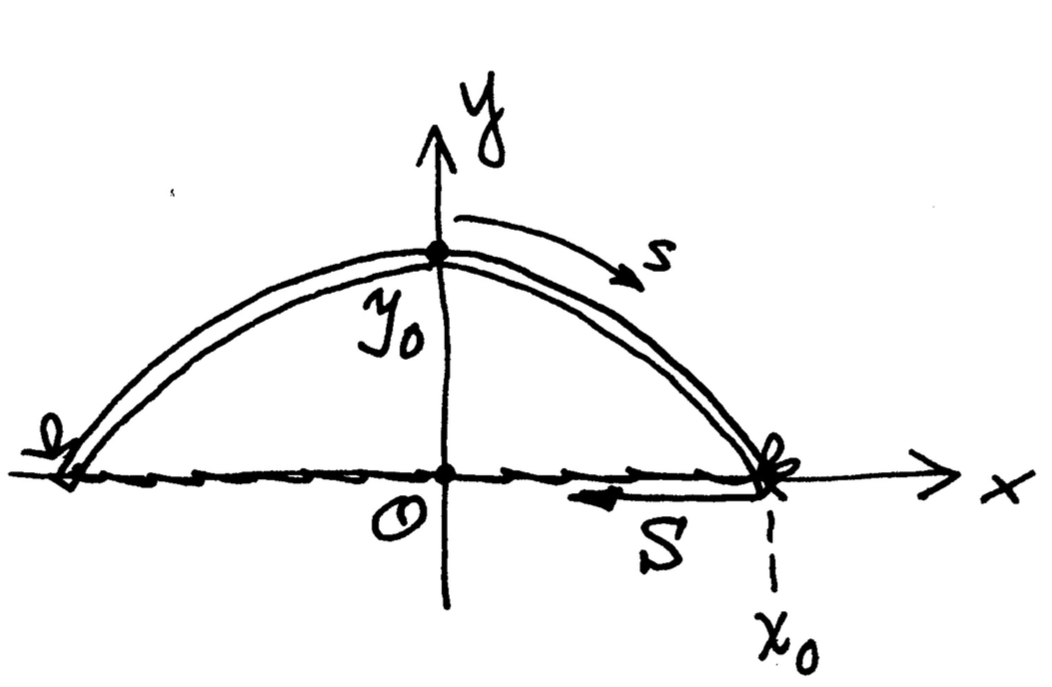
\includegraphics[scale=0.1]{bild.png}
\end{figure}
\begin{equation} \label{eq:original}
	\dfrac{d^2y}{dx^2} + qy \redub{\left(1+\left(\dfrac{dy}{dx}\right)^2\right)^{3/2}}_{\approx 1} = 0 \nonumber
\end{equation}
\begin{equation}
s = \int_0^a{\sqrt{1+y'(x)^2}}=0.5 \nonumber
\end{equation}
\end{frame}

% slide 4
\begin{frame}
\frametitle{Lösning}
\framesubtitle{Förenklat system}
\begin{equation} \label{eq:simplified}
	\dfrac{d^2y}{dx^2} + qy = 0 \nonumber
\end{equation}
\begin{equation}
	y:=e^{rx} \nonumber
\end{equation}
\\
\begin{equation}
 y(x) = A cos(\sqrt{q}\:x)+B sin(\sqrt{q}\:x) \nonumber
\end{equation}
\begin{equation}
 y'(x) = -A\sqrt{q}\: sin(\sqrt{q}\:x) + B\sqrt{q}\:cos(\sqrt{q}\:x) \nonumber
\end{equation}
\end{frame}

% slide 5
\begin{frame}
\frametitle{Lösning}
\framesubtitle{Förenklat system}
\begin{equation} \label{eq:y}
 y(x) = 0.3 cos(\sqrt{q}\:x) \nonumber
\end{equation}
\begin{equation} \label{eq:yprime}
 y'(x) = -0.3\sqrt{q}\: sin(\sqrt{q}\:x) \nonumber
\end{equation}
\begin{equation}
 a = \dfrac{\pi}{2\sqrt{q}} \nonumber
\end{equation}
\end{frame}

% slide 5
\begin{frame}
\frametitle{Lösning}
\framesubtitle{Förenklat system}
Vi söker det $a$ som ger:
\begin{equation}
s = \int_0^a{\sqrt{1+y'(x)^2}}{dx}=0.5 \nonumber
\end{equation}
\usebox{\firstexample}
\end{frame}

% slide 6
\begin{frame}
\frametitle{Lösning}
\framesubtitle{Förenklat system}
Värdet på $a$ finnes iterativt med sekantmetoden:
\begin{equation}
a_n =a_{n-1}-y(a_{n-1})\frac{a_{n-1}-a_{n-2}}{y(a_{n-1})-y(a_{n-2})} \nonumber
\end{equation}
Nu har vi ett värde på $a$ och därmed också $q$ som \textbf{nästan} löser problemet.
\end{frame}

\begin{frame}
\frametitle{Lösning}
\framesubtitle{Ursprungliga problemet}
\begin{equation} \label{eq:original}
	\dfrac{d^2y}{dx^2} + qy \left(1+\left(\dfrac{dy}{dx}\right)^2\right)^{3/2} = 0 \nonumber
\end{equation}
\end{frame}
\begin{frame}
\frametitle{Lösning}
\framesubtitle{Ursprungliga problemet}
\usebox{\findroot}
\usebox{\original}
\end{frame}

\begin{frame}
\frametitle{Lösning}
\framesubtitle{Ursprungliga problemet}
Nu söker vi det q som ger:
\begin{equation}
s = \int{\sqrt{1+y'(x)^2}}{dx}=0.5 \nonumber
\end{equation}
Vi använder \textbf{sekantmetoden} igen.
\end{frame}

\begin{frame}
\frametitle{Lösning}
\framesubtitle{Kraft i bågsträngen}
Vi söker kraften $S$ i bågsträngen:
\begin{figure}[h!]
\centering
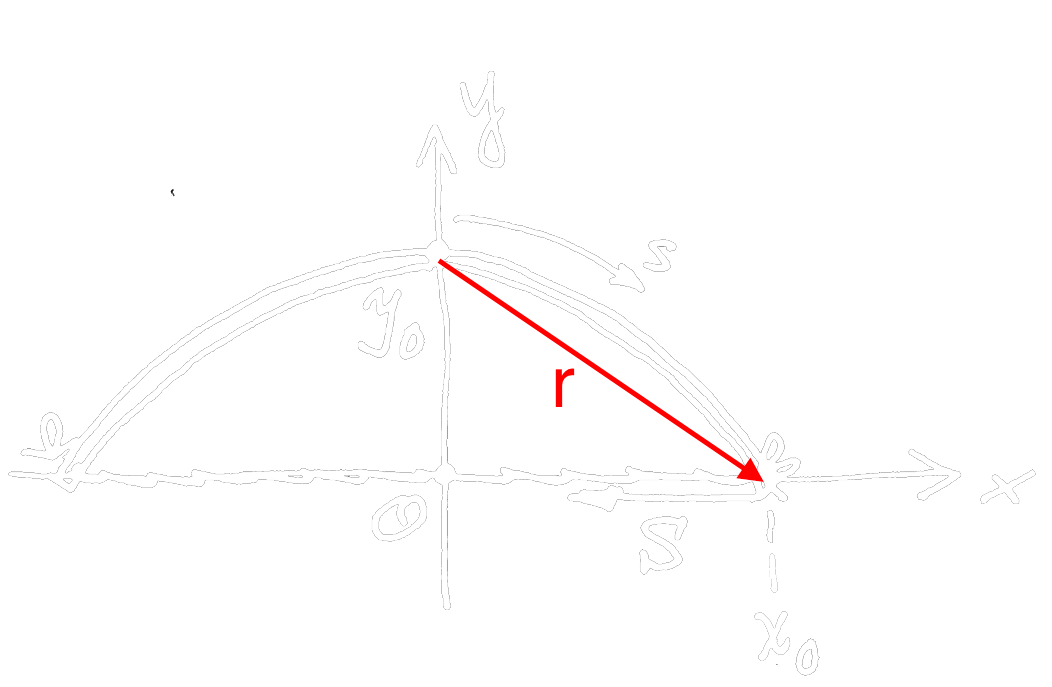
\includegraphics[scale=0.2]{moment.png}
\end{figure}
\begin{equation}
	S \times r(x) = M(x)\nonumber
\end{equation}
\end{frame}

\begin{frame}
\frametitle{Lösning}
\framesubtitle{Kraft i bågsträngen}
\begin{equation}
	S \times r(x) = M(x)\nonumber
\end{equation}
\begin{equation}
	M(x) = -qy(x) \nonumber
\end{equation}
\begin{equation}
	r(x) = \colvec{a}{0} - \colvec{x}{y(x)} \nonumber
\end{equation}
\begin{equation}
	r(x) = -y(x) \quad\quad \textnormal{(ortongonalt mot $S$)} \nonumber
\end{equation}
\begin{equation}
	S = q \nonumber
\end{equation}
\end{frame}

\begin{frame}
\frametitle{Lösning}
\framesubtitle{s som fri variabel}
Differentialen kan istället skrivas med $s$, avståndet från startpunkten längs bågen och \textit{krökningen} i bågen $-qy(s)$
\begin{equation}
	\dfrac{d^2y}{ds^2}+qy\left(\dfrac{dx}{ds}\right)=0, \quad \dfrac{dx}{ds} = \sqrt{1-\left(\dfrac{dy}{ds}\right)^2} \nonumber
\end{equation}
\begin{equation}
s \in [0, 0.5] \nonumber
\end{equation}

\end{frame}

\begin{frame}
\frametitle{Lösning}
\framesubtitle{Tredje ordningens differentialekvation i MATLAB}
\begin{align}
\begin{tabular}{ l l }
	$u_1 = x$ 					& $u_1' = \sqrt{1-\left(u_3\right)^2}$\\
	& \\
	$u_2 = y$ 					& $u_2' = u_3$\\
	& \\
	$u_3 = \dfrac{dy}{ds}$ 		& $u_3' = -qu_2\sqrt{1-\left(u_3\right)^2}$
\end{tabular}
\nonumber
\end{align}
\begin{equation}
s \in [0, 0.5] \nonumber
\end{equation}
\end{frame}

\begin{frame}
\frametitle{Lösning}
\framesubtitle{Sekantmetoden (igen!)}
Nu använder vi återigen \textbf{sekantmetoden} för att lösa differentialen. Denna gång letar vi efter det $q$ som ger ett sista y-värde (från \textit{ode45}) som $y=0$
\end{frame}

\begin{frame}
\frametitle{Tack!}
\framesubtitle{GitHub Implementation! :D}
\centering
\url{https://github.com/christopherL91/Numme14}\\
\href{mailto:vkr@kth.se}{vkr@kth.se}\\
\href{mailto:lillt@kth.se}{lillt@kth.se}
\end{frame}

\end{document}